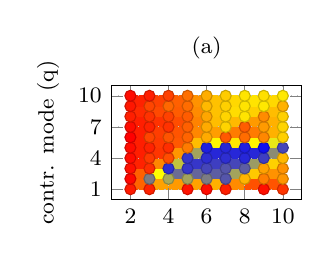
\begin{tikzpicture}
\begin{axis}
[
width=0.33\textwidth,
height=0.25\textwidth,
style={font=\footnotesize},
grid=major,
grid style={dotted},
align=center,
%xlabel={tensor order},
ylabel={contr. mode (q)},
title={{(a)}}, %  bgemm, asymmetric
scaled ticks=false,
zlabel={GFlops},
view={0}{90}, 
ytick={1,4,7,10},
xtick={2,4,6,8,10},
xmin=1, xmax=11,
ymin=0, ymax=11,
try min ticks=8,
zmin=300, zmax=2300,
point meta min=300, point meta max=2300,
colormap/hot, 
samples=50,
%colorbar sampled,
%colorbar/width=0.2cm,
%colorbar style={
%	point meta min=300, point meta max=2300,
%	samples=50,
%	font=\footnotesize,
%	ytick={300,1300,2300},
%	yticklabels={0.3,1.3,2.3},
%	%title={\scriptsize Gflops},
%	%ylabel={\scriptsize Gflops},
%}
]
%\addplot3[mesh, scatter,samples=50,shader=interp]
%\addplot3[only marks, mesh, scatter,scatter src=z,samples=50,] % z buffer=sort, scatter src=z,
\addplot3[contour filled={number=100},scatter,shader=flat,samples=50]
%\addplot3+[mesh,scatter,shader=flat corner,samples=50, only marks, mark size=2]
coordinates{
	
(2.000,1.000,2142.734) (2.000,2.000,2241.014) (2.000,3.000,2205.546) (2.000,4.000,2226.263) (2.000,5.000,2232.877) (2.000,6.000,2281.816) (2.000,7.000,2222.317) (2.000,8.000,2122.831) (2.000,9.000,2166.437) (2.000,10.000,2231.354) 

(3.000,1.000,2104.803) (3.000,2.000,620.292) (3.000,3.000,2053.810) (3.000,4.000,1989.460) (3.000,5.000,2100.108) (3.000,6.000,1923.866) (3.000,7.000,2109.798) (3.000,8.000,2032.918) (3.000,9.000,1931.835) (3.000,10.000,2137.550) 

(4.000,1.000,2303.560) (4.000,2.000,742.055) (4.000,3.000,436.752) (4.000,4.000,1889.266) (4.000,5.000,2050.848) (4.000,6.000,1845.429) (4.000,7.000,2029.757) (4.000,8.000,1947.246) (4.000,9.000,1753.968) (4.000,10.000,1945.836) 

(5.000,1.000,2197.949) (5.000,2.000,727.736) (5.000,3.000,441.734) (5.000,4.000,458.055) (5.000,5.000,1643.657) (5.000,6.000,1763.676) (5.000,7.000,1793.195) (5.000,8.000,1799.906) (5.000,9.000,1726.622) (5.000,10.000,1710.693) 

(6.000,1.000,2225.857) (6.000,2.000,621.489) (6.000,3.000,489.438) (6.000,4.000,435.500) (6.000,5.000,386.554) (6.000,6.000,1410.907) (6.000,7.000,1419.437) (6.000,8.000,1428.795) (6.000,9.000,1330.280) (6.000,10.000,1386.923) 

(7.000,1.000,2137.668) (7.000,2.000,530.662) (7.000,3.000,532.587) (7.000,4.000,439.307) (7.000,5.000,400.923) (7.000,6.000,1835.402) (7.000,7.000,1186.143) (7.000,8.000,1195.514) (7.000,9.000,1211.432) (7.000,10.000,1230.143) 

(8.000,1.000,2411.000) (8.000,2.000,1340.829) (8.000,3.000,546.729) (8.000,4.000,405.255) (8.000,5.000,381.061) (8.000,6.000,1724.053) (8.000,7.000,1816.684) (8.000,8.000,1103.276) (8.000,9.000,1109.365) (8.000,10.000,1119.582) 

(9.000,1.000,2215.896) (9.000,2.000,1637.409) (9.000,3.000,1448.314) (9.000,4.000,477.752) (9.000,5.000,353.959) (9.000,6.000,1596.361) (9.000,7.000,1496.308) (9.000,8.000,1566.431) (9.000,9.000,1085.107) (9.000,10.000,1135.908) 

(10.000,1.000,2011.147) (10.000,2.000,1504.412) (10.000,3.000,1538.421) (10.000,4.000,1335.732) (10.000,5.000,483.993) (10.000,6.000,1202.734) (10.000,7.000,1197.316) (10.000,8.000,1213.834) (10.000,9.000,1362.208) (10.000,10.000,1087.708)


};
\end{axis}
\end{tikzpicture}
\hfill
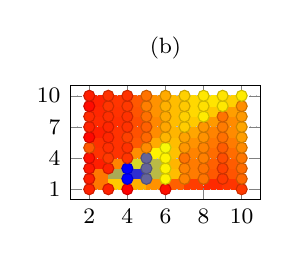
\begin{tikzpicture}
\begin{axis}
[
width=0.33\textwidth,
height=0.25\textwidth,
style={font=\footnotesize},
grid=major,
grid style={dotted},
align=center,
%xlabel={tensor order},
%ylabel={contr. mode (q)},
title={{(b)}}, %  ompfor<2d-slice> ttm<par-loops,seq-blas,$q$-slice>, asymmetric
scaled ticks=false,
zlabel={GFlops},
view={0}{90}, 
%view={-45}{45}, 
ytick={1,4,7,10},
xtick={2,4,6,8,10},
xmin=1, xmax=11,
ymin=0, ymax=11,
try min ticks=8,
zmin=300, zmax=2300,
point meta min=300, point meta max=2300,
colormap/hot, 
samples=50,
%colorbar sampled,
%colorbar/width=0.2cm,
%colorbar style={
%	point meta min=300, point meta max=2300,
%	samples=50,
%	font=\footnotesize,
%	ytick={300,1300,2300},
%	yticklabels={0.3,1.3,2.3},
%	%title={\scriptsize Gflops},
%	%ylabel={\scriptsize Gflops},
%}
]
%\addplot3[mesh, scatter,samples=50,shader=interp]
%\addplot3[only marks, mesh, scatter,scatter src=z,samples=50,] % z buffer=sort, scatter src=z,
\addplot3[contour filled={number=100},scatter,shader=flat,samples=50]
%\addplot3+[mesh,scatter,shader=flat corner,samples=50, only marks, mark size=2]
coordinates{

(2.000,1.000,2107.002) (2.000,2.000,2127.162) (2.000,3.000,2176.298) (2.000,4.000,2215.649) (2.000,5.000,1837.632) (2.000,6.000,2241.609) (2.000,7.000,2101.558) (2.000,8.000,2075.436) (2.000,9.000,2236.130) (2.000,10.000,2133.353) 

(3.000,1.000,2119.523) (3.000,2.000,167.437) (3.000,3.000,2112.420) (3.000,4.000,1989.285) (3.000,5.000,2041.921) (3.000,6.000,2084.201) (3.000,7.000,2080.454) (3.000,8.000,2046.614) (3.000,9.000,2013.009) (3.000,10.000,2024.421) 

(4.000,1.000,2285.299) (4.000,2.000,314.287) (4.000,3.000,311.849) (4.000,4.000,2011.869) (4.000,5.000,2039.029) (4.000,6.000,1944.642) (4.000,7.000,2023.178) (4.000,8.000,2033.385) (4.000,9.000,1992.379) (4.000,10.000,2039.303) 

(5.000,1.000,2475.804) (5.000,2.000,568.291) (5.000,3.000,562.230) (5.000,4.000,562.587) (5.000,5.000,1564.667) (5.000,6.000,1756.890) (5.000,7.000,1791.524) (5.000,8.000,1712.024) (5.000,9.000,1626.887) (5.000,10.000,1695.764) 

(6.000,1.000,2218.038) (6.000,2.000,1025.980) (6.000,3.000,1034.039) (6.000,4.000,1026.350) (6.000,5.000,945.367) (6.000,6.000,1340.191) (6.000,7.000,1422.937) (6.000,8.000,1402.244) (6.000,9.000,1375.707) (6.000,10.000,1411.432) 

(7.000,1.000,2307.246) (7.000,2.000,1602.074) (7.000,3.000,1617.348) (7.000,4.000,1682.539) (7.000,5.000,1516.443) (7.000,6.000,1446.511) (7.000,7.000,1229.353) (7.000,8.000,1202.606) (7.000,9.000,1245.855) (7.000,10.000,1211.880) 

(8.000,1.000,2441.539) (8.000,2.000,1699.771) (8.000,3.000,1686.405) (8.000,4.000,1622.372) (8.000,5.000,1600.438) (8.000,6.000,1530.707) (8.000,7.000,1508.466) (8.000,8.000,1073.808) (8.000,9.000,1123.363) (8.000,10.000,1096.486) 

(9.000,1.000,2330.060) (9.000,2.000,1985.056) (9.000,3.000,1941.312) (9.000,4.000,1892.533) (9.000,5.000,1805.699) (9.000,6.000,1706.515) (9.000,7.000,1658.818) (9.000,8.000,1693.350) (9.000,9.000,1093.684) (9.000,10.000,1112.530) 

(10.000,1.000,1988.818) (10.000,2.000,1750.516) (10.000,3.000,1728.226) (10.000,4.000,1678.568) (10.000,5.000,1576.395) (10.000,6.000,1476.492) (10.000,7.000,1429.733) (10.000,8.000,1496.574) (10.000,9.000,1557.162) (10.000,10.000,1068.719) 


};
\end{axis}
\end{tikzpicture}
\hfill
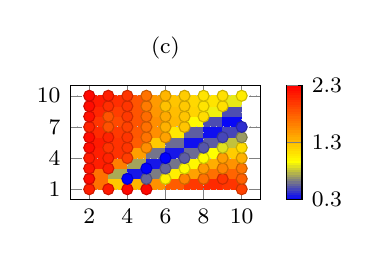
\begin{tikzpicture}
\begin{axis}
[
width=0.33\textwidth,
height=0.25\textwidth,
style={font=\footnotesize},
grid=major,
grid style={dotted},
align=center,
%xlabel={tensor order},
%ylabel={contr. mode (q)},
title={{(c)}}, %  ompfor<qd-slice> ttm<par-loops,seq-blas,$q$-slice>, asymmetric
scaled ticks=false,
zlabel={GFlops},
view={0}{90}, 
%view={-45}{45}, 
ytick={1,4,7,10},
xtick={2,4,6,8,10},
%xmin=2, xmax=10,
%ymin=1, ymax=10,
xmin=1, xmax=11,
ymin=0, ymax=11,
try min ticks=8,
zmin=300, zmax=2300,
point meta min=300, point meta max=2300,
%colormap/jet, 
colormap/hot, 
%colormap/blackwhite,
%colormap={whiteblack}{indices of colormap={\pgfplotscolormaplastindexof{blackwhite},...,0 of blackwhite}},
samples=50,
%colormap access=piecewise const,
colorbar sampled,
colorbar/width=0.2cm,
colorbar style={
	point meta min=300, point meta max=2300,
	samples=50,
	font=\footnotesize,
	ytick={300,1300,2300},
	yticklabels={0.3,1.3,2.3},
	%title={\scriptsize Gflops},
	%ylabel={\scriptsize Gflops},
}
]
%\addplot3[mesh, scatter,samples=50,shader=interp]
%\addplot3[only marks, mesh, scatter,scatter src=z,samples=50,] % z buffer=sort, scatter src=z,
\addplot3[contour filled={number=100},scatter,shader=flat,samples=50]
%\addplot3+[mesh,scatter,shader=flat corner,samples=50, only marks, mark size=2]
coordinates{

(2.000,1.000,2134.021) (2.000,2.000,2224.864) (2.000,3.000,2184.477) (2.000,4.000,2142.541) (2.000,5.000,2229.439) (2.000,6.000,2238.772) (2.000,7.000,2105.091) (2.000,8.000,2201.214) (2.000,9.000,2232.448) (2.000,10.000,2240.926) 

(3.000,1.000,2146.896) (3.000,2.000,167.544) (3.000,3.000,2121.476) (3.000,4.000,2105.304) (3.000,5.000,2027.717) (3.000,6.000,2104.722) (3.000,7.000,1866.561) (3.000,8.000,1855.180) (3.000,9.000,2041.894) (3.000,10.000,2122.692) 

(4.000,1.000,2244.985) (4.000,2.000,313.766) (4.000,3.000,167.879) (4.000,4.000,1973.457) (4.000,5.000,2013.391) (4.000,6.000,2010.678) (4.000,7.000,1949.136) (4.000,8.000,1989.844) (4.000,9.000,2017.192) (4.000,10.000,2015.899) 

(5.000,1.000,2250.694) (5.000,2.000,574.277) (5.000,3.000,315.908) (5.000,4.000,166.343) (5.000,5.000,1559.782) (5.000,6.000,1688.138) (5.000,7.000,1711.412) (5.000,8.000,1721.389) (5.000,9.000,1653.587) (5.000,10.000,1691.902) 

(6.000,1.000,2403.465) (6.000,2.000,1026.371) (6.000,3.000,576.699) (6.000,4.000,312.020) (6.000,5.000,160.917) (6.000,6.000,1443.174) (6.000,7.000,1370.699) (6.000,8.000,1414.204) (6.000,9.000,1283.900) (6.000,10.000,1351.446) 

(7.000,1.000,2305.894) (7.000,2.000,1613.830) (7.000,3.000,988.435) (7.000,4.000,554.792) (7.000,5.000,290.305) (7.000,6.000,157.356) (7.000,7.000,1270.432) (7.000,8.000,1266.914) (7.000,9.000,1255.620) (7.000,10.000,1224.914) 

(8.000,1.000,2437.239) (8.000,2.000,1706.219) (8.000,3.000,1489.110) (8.000,4.000,999.755) (8.000,5.000,531.137) (8.000,6.000,280.182) (8.000,7.000,148.892) (8.000,8.000,1156.621) (8.000,9.000,1110.478) (8.000,10.000,1116.944) 

(9.000,1.000,2355.395) (9.000,2.000,2003.839) (9.000,3.000,1603.752) (9.000,4.000,1477.309) (9.000,5.000,887.839) (9.000,6.000,492.554) (9.000,7.000,262.294) (9.000,8.000,150.408) (9.000,9.000,1129.997) (9.000,10.000,1121.143) 

(10.000,1.000,1944.959) (10.000,2.000,1789.054) (10.000,3.000,1665.441) (10.000,4.000,1375.291) (10.000,5.000,1147.731) (10.000,6.000,715.205) (10.000,7.000,422.658) (10.000,8.000,236.076) (10.000,9.000,136.520) (10.000,10.000,1078.495) 


};
\end{axis}
\end{tikzpicture}


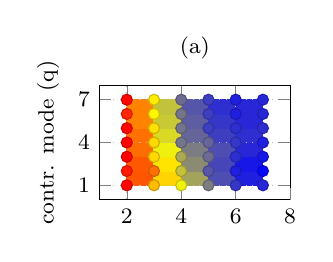
\begin{tikzpicture}
\begin{axis}
[
width=0.33\textwidth,
height=0.25\textwidth,
style={font=\footnotesize},
grid=major,
grid style={dotted},
align=center,
%xlabel={tensor order},
ylabel={contr. mode (q)},
title={{(a)}}, %  bgemm, asymmetric
scaled ticks=false,
zlabel={GFlops},
view={0}{90}, 
ytick={1,4,7,10},
xtick={2,4,6,8},
xmin=1, xmax=8,
ymin=0, ymax=8,
try min ticks=8,
zmin=0, zmax=2600,
point meta min=0, point meta max=2600,
colormap/hot, 
samples=50,
%colorbar sampled,
%colorbar/width=0.2cm,
%colorbar style={
%	point meta min=300, point meta max=2300,
%	samples=50,
%	font=\footnotesize,
%	ytick={300,1300,2300},
%	yticklabels={0.3,1.3,2.3},
%	%title={\scriptsize Gflops},
%	%ylabel={\scriptsize Gflops},
%}
]
%\addplot3[mesh, scatter,samples=50,shader=interp]
%\addplot3[only marks, mesh, scatter,scatter src=z,samples=50,] % z buffer=sort, scatter src=z,
\addplot3[contour filled={number=100},scatter,shader=flat,samples=50]
%\addplot3+[mesh,scatter,shader=flat corner,samples=50, only marks, mark size=2]
coordinates{

(2.000,1.000,2527.923) (2.000,2.000,2398.051) (2.000,3.000,2573.521) (2.000,4.000,2570.296) (2.000,5.000,2540.651) (2.000,6.000,2326.903) (2.000,7.000,2545.629) 

(3.000,1.000,1312.517) (3.000,2.000,1835.211) (3.000,3.000,1133.124) (3.000,4.000,1120.384) (3.000,5.000,1066.704) (3.000,6.000,915.932) (3.000,7.000,997.168) 

(4.000,1.000,825.045) (4.000,2.000,655.270) (4.000,3.000,579.750) (4.000,4.000,390.794) (4.000,5.000,411.134) (4.000,6.000,409.619) (4.000,7.000,375.457) 

(5.000,1.000,420.343) (5.000,2.000,308.678) (5.000,3.000,377.118) (5.000,4.000,348.232) (5.000,5.000,216.877) (5.000,6.000,232.073) (5.000,7.000,218.457) 

(6.000,1.000,206.774) (6.000,2.000,119.299) (6.000,3.000,167.691) (6.000,4.000,183.571) (6.000,5.000,179.989) (6.000,6.000,126.876) (6.000,7.000,128.135) 

(7.000,1.000,150.823) (7.000,2.000,33.170) (7.000,3.000,83.979) (7.000,4.000,128.221) (7.000,5.000,157.368) (7.000,6.000,143.557) (7.000,7.000,133.647) 


};
\end{axis}
\end{tikzpicture}
\hfill
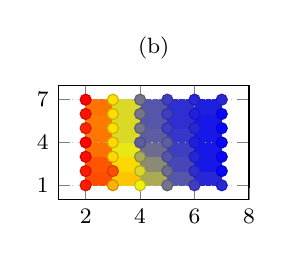
\begin{tikzpicture}
\begin{axis}
[
width=0.33\textwidth,
height=0.25\textwidth,
style={font=\footnotesize},
grid=major,
grid style={dotted},
align=center,
%xlabel={tensor order},
%ylabel={contr. mode (q)},
title={{(b)}}, %  ompfor<2d-slice> ttm<par-loops,seq-blas,$q$-slice>, asymmetric
scaled ticks=false,
zlabel={GFlops},
view={0}{90}, 
%view={-45}{45}, 
ytick={1,4,7,10},
xtick={2,4,6,8},
xmin=1, xmax=8,
ymin=0, ymax=8,
try min ticks=8,
zmin=0, zmax=2600,
point meta min=0, point meta max=2600,
colormap/hot, 
samples=50,
%colorbar sampled,
%colorbar/width=0.2cm,
%colorbar style={
%	point meta min=300, point meta max=2300,
%	samples=50,
%	font=\footnotesize,
%	ytick={300,1300,2300},
%	yticklabels={0.3,1.3,2.3},
%	%title={\scriptsize Gflops},
%	%ylabel={\scriptsize Gflops},
%}
]
%\addplot3[mesh, scatter,samples=50,shader=interp]
%\addplot3[only marks, mesh, scatter,scatter src=z,samples=50,] % z buffer=sort, scatter src=z,
\addplot3[contour filled={number=100},scatter,shader=flat,samples=50]
%\addplot3+[mesh,scatter,shader=flat corner,samples=50, only marks, mark size=2]
coordinates{

(2.000,1.000,2394.429) (2.000,2.000,2411.386) (2.000,3.000,2508.441) (2.000,4.000,2549.390) (2.000,5.000,2334.831) (2.000,6.000,2454.725) (2.000,7.000,2556.685) 

(3.000,1.000,1395.054) (3.000,2.000,2055.946) (3.000,3.000,1121.102) (3.000,4.000,1120.659) (3.000,5.000,1089.377) (3.000,6.000,1102.959) (3.000,7.000,1078.957) 

(4.000,1.000,819.991) (4.000,2.000,729.342) (4.000,3.000,579.869) (4.000,4.000,334.133) (4.000,5.000,390.153) (4.000,6.000,407.045) (4.000,7.000,394.057) 

(5.000,1.000,414.803) (5.000,2.000,369.532) (5.000,3.000,295.077) (5.000,4.000,318.473) (5.000,5.000,209.139) (5.000,6.000,214.825) (5.000,7.000,223.888) 

(6.000,1.000,208.097) (6.000,2.000,156.950) (6.000,3.000,141.868) (6.000,4.000,119.992) (6.000,5.000,134.757) (6.000,6.000,126.271) (6.000,7.000,133.034) 

(7.000,1.000,151.228) (7.000,2.000,27.225) (7.000,3.000,30.634) (7.000,4.000,31.221) (7.000,5.000,30.322) (7.000,6.000,31.152) (7.000,7.000,133.496) 


};
\end{axis}
\end{tikzpicture}
\hfill
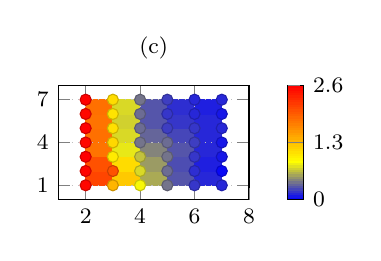
\begin{tikzpicture}
\begin{axis}
[
width=0.33\textwidth,
height=0.25\textwidth,
style={font=\footnotesize},
grid=major,
grid style={dotted},
align=center,
%xlabel={tensor order},
%ylabel={contr. mode (q)},
title={{(c)}}, %  ompfor<qd-slice> ttm<par-loops,seq-blas,$q$-slice>, asymmetric
scaled ticks=false,
zlabel={GFlops},
view={0}{90}, 
ytick={1,4,7,10},
xtick={2,4,6,8},
xmin=1, xmax=8,
ymin=0, ymax=8,
try min ticks=8,
zmin=0, zmax=2600,
point meta min=0, point meta max=2600,
%colormap/jet, 
colormap/hot, 
%colormap/blackwhite,
%colormap={whiteblack}{indices of colormap={\pgfplotscolormaplastindexof{blackwhite},...,0 of blackwhite}},
samples=50,
%colormap access=piecewise const,
colorbar sampled,
colorbar/width=0.2cm,
colorbar style={
point meta min=0, point meta max=2600,
samples=50,
font=\footnotesize,
ytick={0,1300,2600},
yticklabels={0,1.3,2.6},
%title={\scriptsize Gflops},
%ylabel={\scriptsize Gflops},
}
]
%\addplot3[mesh, scatter,samples=50,shader=interp]
%\addplot3[only marks, mesh, scatter,scatter src=z,samples=50,] % z buffer=sort, scatter src=z,
\addplot3[contour filled={number=100},scatter,shader=flat,samples=50]
%\addplot3+[mesh,scatter,shader=flat corner,samples=50, only marks, mark size=2]
coordinates{

(2.000,1.000,2536.639) (2.000,2.000,2549.050) (2.000,3.000,2598.729) (2.000,4.000,2525.744) (2.000,5.000,2590.830) (2.000,6.000,2544.134) (2.000,7.000,2589.762) 

(3.000,1.000,1375.656) (3.000,2.000,2048.636) (3.000,3.000,1013.687) (3.000,4.000,1124.134) (3.000,5.000,1075.977) (3.000,6.000,1052.382) (3.000,7.000,1098.544) 

(4.000,1.000,833.978) (4.000,2.000,732.322) (4.000,3.000,660.833) (4.000,4.000,413.827) (4.000,5.000,368.029) (4.000,6.000,382.244) (4.000,7.000,404.286) 

(5.000,1.000,415.086) (5.000,2.000,368.007) (5.000,3.000,411.465) (5.000,4.000,371.633) (5.000,5.000,212.971) (5.000,6.000,198.100) (5.000,7.000,222.798) 

(6.000,1.000,206.159) (6.000,2.000,156.941) (6.000,3.000,192.783) (6.000,4.000,217.075) (6.000,5.000,186.601) (6.000,6.000,132.454) (6.000,7.000,130.229) 

(7.000,1.000,150.869) (7.000,2.000,27.399) (7.000,3.000,91.695) (7.000,4.000,85.698) (7.000,5.000,132.060) (7.000,6.000,86.740) (7.000,7.000,146.783) 


};
\end{axis}
\end{tikzpicture}
